\usetikzlibrary{calc}
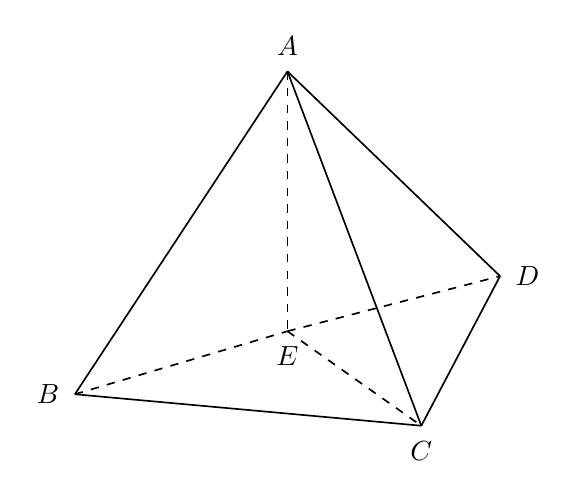
\begin{tikzpicture}[line width=0.6pt, >=stealth, font=\normalsize]
  \coordinate (A) at (0,3.4);
  \coordinate (E) at (0,0.1);
  \coordinate (B) at (-2.7,-0.7);
  \coordinate (C) at (1.7,-1.1);
  \coordinate (D) at (2.7,0.8);
  % visible solid edges
  \draw[solid] (A) -- (B);
  \draw[solid] (B) -- (C);
  \draw[solid] (C) -- (D);
  \draw[solid] (A) -- (D);
  \draw[solid] (A) -- (C);
  % hidden dashed edges
  \draw[dashed] (A) -- (E);
  \draw[dashed] (B) -- (E);
  \draw[dashed] (E) -- (D);
  \draw[dashed] (E) -- (C);
  \node[above=2pt] at (A) {$A$};
  \node[left=2pt] at (B) {$B$};
  \node[below=2pt] at (C) {$C$};
  \node[right=2pt] at (D) {$D$};
  \node[below=2pt] at (E) {$E$};
\end{tikzpicture}
